\chapter{Appendix}
\label{chap:appendix}

%%% TODO: Put a caption to it
\begin{lstlisting}[label=lst:brave-report, caption=Brave Browser telemetry questions]
\end{lstlisting}
\begin{enumerate}
    \label{list:brave_question}
    \item How long has this browser been open for the last seven days?
    \item Have you made Brave your default browser?
    \item Did you follow the on-boarding process
    \item Did you import settings and bookmarks, and if so from where?
    \item How many bookmarks do you have?
    \item How many open windows do you have?
    \item How many open tabs do you have?
    \item What has been your interaction with the shields icon?
    \item Have you ever used a private window?
    \item Have you ever used a Tor private window?
    \item What is the state of your Brave Rewards wallet? [NOT IMPLEMENTED]
    \item How much BAT, excluding grants, is in your wallet?
    \item  Have you made use of Auto-contribute in Brave Rewards?
    \item Have you made use of tips within Brave Rewards?
    \item Have you enabled sync?
    \item How many extensions have you installed?
    \item Have you enabled Brave Ads?
    \item How many questions the browser was able to answer within a week?
    \item How many times did you search last week?
    \item Which is your currently selected search engine?
    \item How much data did Brave save you last week?
    \item Is crash reporting enabled?
    \item Have you used SpeedReader?
    \item Number of times user clicked on SpeedReader button to toggle the feature?
    \item On average, how many New Tab Pages did you create per day?
    \item Is the sponsored new tab page option enabled?
    \item On average, how many of the New Tab Pages you saw per day were sponsored?
    \item On the New Tab Page, did you click the Customize Settings icon?
\end{enumerate}


\newpage

\begin{lstlisting}[label=lst:ubuntu-report, caption=Example report for an Ubuntu X86\_64 System\cite{roche_ubuntuubuntu-report_2020}]
{
  "Version": "18.04",
  "OEM": {
    "Vendor": "Vendor Name",
    "Product": "4287CTO"
  },
  "BIOS": {
    "Vendor": "Vendor Name",
    "Version": "8DET52WW (1.27)"
  },
  "CPU": {
    "OpMode": "32-bit, 64-bit",
    "CPUs": "8",
    "Threads": "2",
    "Cores": "4",
    "Sockets": "1",
    "Vendor": "Genuine",
    "Family": "6",
    "Model": "158",
    "Stepping": "10",
    "Name": "Intius Corus i5-8300H CPU @ 2.30GHz",
    "Virtualization": "VT-x"
  },
  "Arch": "amd64",
  "GPU": [
    {
      "Vendor": "8086",
      "Model": "0126"
    }
  ],
  "RAM": 8,
  "Disks": [
    240.1,
    500.1
  ],
  "Partitions": [
    229.2,
    479.7
  ],
  "Screens": [
    {
      "Size": "277mmx156mm",
      "Resolution": "1366x768",
      "Frequency": "60.02"
    },
    {
      "Resolution": "1920x1080",
      "Frequency": "60.00"
    }
  ],
  "Autologin": false,
  "LivePatch": true,
  "Session": {
    "DE": "ubuntu:GNOME",
    "Name": "ubuntu",
    "Type": "x11"
  },
  "Language": "fr_FR",
  "Timezone": "Europe/Paris",
  "Install": {
    "Media": "Ubuntu 18.04 LTS \"Bionic Beaver\" - Alpha amd64 (20180305)",
    "Type": "GTK",
    "PartitionMethod": "use_device",
    "DownloadUpdates": true,
    "Language": "fr",
    "Minimal": false,
    "RestrictedAddons": false,
    "Stages": {
      "0": "language",
      "3": "language",
      "10": "console_setup",
      "15": "prepare",
      "25": "partman",
      "27": "start_install",
      "37": "timezone",
      "49": "usersetup",
      "57": "user_done",
      "829": "done"
    }
  }
}
\end{lstlisting}

\newpage
\begin{figure}
    \centering
    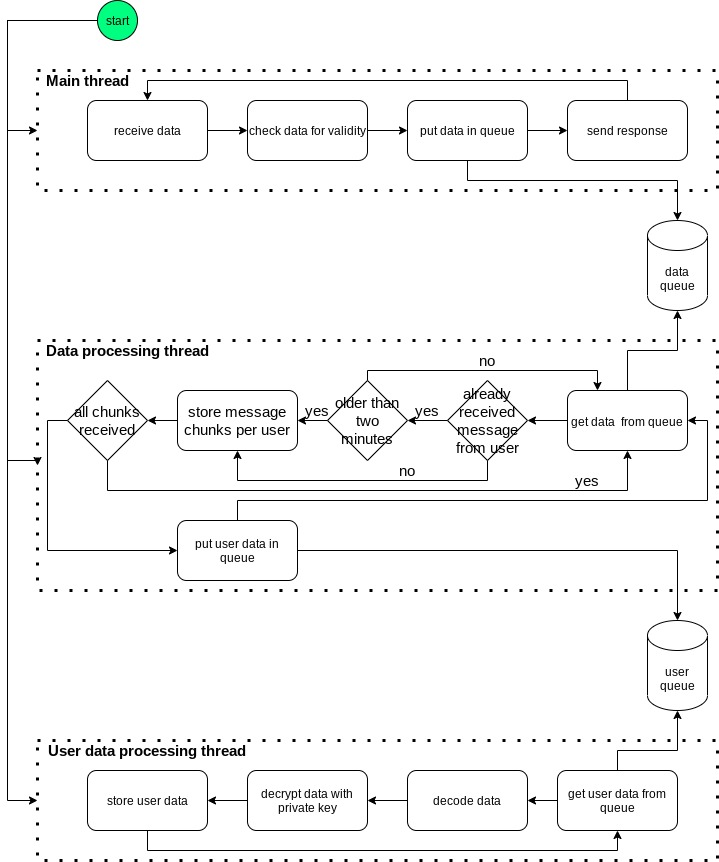
\includegraphics[width=\textwidth]{latex/figures/server_proc.jpg}
    \caption{Simplified overview of the server's concurrent threads}
    \label{fig:server_proc}
\end{figure}
